\documentclass[a4paper, twoside, 12pt]{report}
\usepackage{graphicx}
\usepackage{titling}
\usepackage[a4paper, margin=1in]{geometry}
\usepackage{listings}
\lstset{breaklines}

% font?
\title{N-Player Durak with Artificial Intelligence}
\author{Seyhan Van Khan}
\date{June 2024}
\makeatletter

\begin{document}


\begin{titlepage}
	\centering
	{\Huge \@title}
	\vspace{1cm}

	
\includegraphics[width=5cm]{./imperial.png}
	\vspace{1cm} \\
	{\large  Imperial College London} \\
	\vspace{.4cm}
	{\large  Department of Computing} \\
	\vspace{.4cm}
	{\large  Bachelor of Engineering Final Year Project} \\
	\vspace{1cm}
	{\Huge  Seyhan Van Khan} \\
	\vspace{4cm}
	{\Large  Supervisor: Nicholas Wu} \\
	\vspace{0.5cm}
	{\Large  Second Marker: Benjamin Hou} \\
	\vspace{1cm}
	{\Large \@date}
\end{titlepage}

\renewcommand{\abstractname}{Acknowledgements}
\begin{abstract}

	I would like to thank my supervisor, Nicholas Wu, for his time and guidance. As an ex-world record holder of the longest Beggar-My-Neighbour card game, his veteran experience and enthusiasm was incredibly valuable.

	This project also wouldn't be possible without my friend Alex, who got me hooked onto Durak 5 years ago, over many school lunch breaks.

\end{abstract}


\renewcommand{\abstractname}{Ethical Discussion}
\begin{abstract}
	While Durak has not been a target of major investment, similar games have a significant amount of capital and labour spent on it. Other turn-based games like Chess and similarly imperfect-information games like Poker can be studied to find where the ethical discussion goes, if Durak ever grows.

	When enormously expensive AI projects for prominent games emerge, it raises ethical concerns. DeepMind's AlphaZero used thousands of Tensor Processing Units to reach a ``superhuman level of play'' in Chess\cite{alphazero}. It was an incredible advancement to let the algorithm teach itself non-trivial tasks from tabula rasa, but such a sizeable investment is not accessible to most.

	Large AI systems demand a substantial energy consumption, predominantly from non-renewable sources, contributing to carbon emissions and environmental degradation. The mining and processing of materials for hardware components further exacerbate these concerns.

	These investments divert resources from other societal needs. The work on a ``superhuman AI for heads-up no-limit poker'', called Libratus, was funded by grants from Facebook, Carnegie Mellon University, the National Science Foundation, and the U.S. Army Research Office\cite{brown2018}. Balancing AI development with essential sectors like healthcare and education requires careful ethical deliberation and governance.

	Durak is, however, not as huge as games like Chess or Poker. Before 2023, the author found Durak strategies only in GitHub repositories. It was only last year when two unpublished works emerged from 2 sets of university students\cite{azamat}\cite{durakMonteCarlo}. The ethical concerns mentioned would therefore be of little concern, for now.
\end{abstract}

\tableofcontents
\listoffigures
\listoftables


\chapter{Introduction}

Consider a game of Texas Hold'em Poker. At first glance, it appears shrouded in chance. Extremely limited information, bluffing, and the need for luck makes it feel purely random. It was considered the big challenge problem for imperfect-information games. Yet, beneath the randomness lies a world of strategic depth when researchers at Carnegie Mellon University broke that expectation and outperformed the top Poker professionals\cite{brown2018}. It was even able to replicate the human intuition of bluffing.

Could there be strategies to break other seemingly simple card games? This paper explores this question for the card game of Durak. It's a trick-taking game with a rich history in Eastern Europe. As the most popular card game in Russia, dating back to the 18th century\cite{penguin}, it is nevertheless an under-researched area and offers a rich strategic landscape to explore.

Played with 2--6 people and usually 36 cards from a 52-card deck, the aim is to get rid of all your cards. The last player left with cards is the loser, the Durak. The most common variant is Podkidnoy Durak, which is what will be explored in this paper. The variants, however, vary slightly and the code that will simulate Podkidnoy could be tweaked to match the rules.

In each bout, a player attacks his neighbour with any amount of cards with the same value (e.g., two Queens, three Eights). Their neighbour, the defender, will attempt to defend each attack by placing a higher-ranked card of the same suit (or trump suit\footnote{A trump suit is a randomly decided suit (Hearts, Spades, Clubs, or Diamonds) that can defend any other suit.}). If they're unable or refuse to defend, the defender takes all the cards involved in the battle and skips their turn to attack. However, if all are defended, they discard these cards and the ex-defender now attacks their neighbour. If there are still cards in the talon, players fill up until each has at least 6. This clockwise run of attacks continue until there is only 1 player left, considered the loser. Everyone else is considered to have won.

Deciding if an attack can be answered is NP-hard. Even with two players and perfect information, finding optimal moves are hard and is PSPACE-complete to determine you have a winning strategy\cite{bonnet}. Durak is a strategic game of imperfect information and is partially non-deterministic. Starting cards are randomly dealt and player’s hands are hidden from others, except for what’s revealed during attacks.

The notion of only 1 loser, with everyone else a winner poses a unique problem for game strategies. This paper will explore this through analysing n-player games, and use several algorithms to prove whether n-player games are luck-based. N-player means less control in attack sequences and less card drawing to help players. The talon is light with more people, and will be empty with 6 players. The rule of only 36 cards isn't mandatory, so could a higher amount help reduce the luck of player's starting cards? Ultimately, this paper will compare the effectiveness of a skilled player against a random mover to see what strategic thinking offers significant advantages.

\section{Objectives}
This project's objective is to build an environment to then implement and test the best possible strategies to play an n-player game of Durak on a home computer. It can be broken down into these 2 goals.

\begin{enumerate}
	\item Develop a functional implementation of the card game Durak for n players. This will serve as the environment to test the algorithm's strategies. The game should be both memory and time efficient, as well as simple enough to expand for other variants, to ensure optimal performance and ease of testing the agents.
	\item Explore and compare several agents, including a rule-based heuristic, random, and \(max^n\). The agents should run fast enough on standard computers to be accessible to everyone for easy use.
\end{enumerate}

Such an agent should be able to evaluate a move and suggest alternatives. A game of imperfect information and a non-deterministic style makes it an interesting project to determine the best possible strategy. Every human player has a different heuristic rule, a personal strategy that may or may not be the most optimal.

\section{Challenges}
To date, research on the game of Durak has been scarce, particularly at the n-player level. In 2016, Bonnet broke new ground with the first scholarly paper\cite{bonnet} to mention Durak. The proceedings showed that any 2-player game's position (with perfect-information) can be solved in polynomial time. Deciding if an attack could be defended in the same circumstances was, however, shown to be NP-hard. It implies determining computationally feasible strategies for Durak could be exceptionally challenging.

Most studies (mostly random GitHub repositories) have focused on the two-player version of the game. Notably, there is only one non-peer-reviewed paper that explores the n-player dynamics of Durak\cite{durakMonteCarlo}, highlighting a significant gap in the existing literature. This project's objective of creating an environment to implement and test optimal strategies in an n-player Durak game is therefore novel and interesting to look into.

\chapter{Background}

When starting this project, the first place to look was at existing work on the game. Last year, Zarlykov\cite{azamat} investigated the two-player variant, exploring various strategies from random to Monte Carlo Tree Search (MCTS) for the highest win rate against humans. His findings lay good groundwork for an analysis into one-on-one games. The MCTS agent consistently beat the other agents while minimax came second, although there wasn't enough investigation into different search depths. Zarlykov also proves that every game must end, as there is no repetition of state in Durak. When the attacker places their attacking cards, they must either end up discarded or in the defender's hand. The same reasoning can be applied to n-player Durak, as when cards reach another hand, the defender is skipped, and so unable to send the cards back to repeat a game state. No infinite loops guarantee the search space can't be revisited.

Tang et al\cite{durakMonteCarlo} shows how a Monte Carlo Tree Search could work for 4-players. Their research tackled the challenge of creating a competitive AI for the more complex 4-player variant of Durak. By employing a Monte Carlo Tree Search (MCTS) algorithm, Tang et al\. explored strategies for navigating the larger decision space of multiple players. There is however a considerably large number of iterations involved. Their solution takes a lot of time to simulate and back-propagate, as well as not use all the information given. The algorithm also only uses heuristics on what kinds of cards are in what hands, as opposed to the exact cards. They also could not show whether the unpredictable nature of Durak could be stopped for the agent win every time.

Shannon's groundbreaking work on ``Programming a Computer for Playing Chess'' in 1949 laid the groundwork for modern Chess-playing AI\cite{shannon}. While computing power was extremely limited then, he proposed a theoretical approach for evaluating chess positions and choosing the best move. This concept was novel to Chess and although not a complete algorithm, could be used for Durak.  While Shannon's work doesn't directly address card games, it introduces the minimax principle, which evaluates possible future game states based on their desirability and your opponent's potential moves. This framework can be adapted to analyse card game possibilities and inform your Durak algorithm.

The paper ``An Algorithmic Solution of N-Person Games'' proposes the \(max^n\) algorithm for finding an equilibrium point n-person games of perfect information\cite{luckhart}. Instead of a minimax approach like Shannon's and its single value, Luckhart adapts the procedure for a vector of payoff values for each player, for each node in the game tree. This algorithm analyses the entire game tree to find an equilibrium point, which is a set of strategies for each player that offers the best expected outcome considering what other players might do. The paper, however, doesn't address how well \(max^n\) scales with complex games or the computational cost it incurs in imperfect-information games. Understanding these limitations can help assess its applicability to Durak. With no initial knowledge of starting cards, the number of initial responses to moves would make the game tree significantly larger. The attacker has 6 cards to choose from, but would have to evaluate every combination of 6 cards from the 30 left. \(^30 C_6\) combinations means each player's initial set of cards comes from a pool of 593,775 possible combinations

\chapter{Creating the Game}

The first objective is to create a solid framework to run games of Durak on, that is tailored for efficient evaluation. It should be easily adaptable for different variants with different card amounts.

\section{The Tech Stack}

When selecting a language to analyse AI for Durak, there are several key motivations.

\begin{enumerate}
	\item Functional Programming: To effectively analyse with search and recursion, a functional paradigm is ideal. They emphasise immutability, pure functions and a declarative style, leading to code that is concise and self-explanatory with no side effects.
	\item Static typing: minimise runtime errors and code maintainability.
\end{enumerate}

Given these principles, Haskell is the compelling choice and thus will be the language to produce the work in.

\section{Structure}

To manage dependencies, Stack\cite{hstack} will be the chosen framework to build the game.

\subsection{Cards}

To represent the foundation of a card game, we need certain data types defined.

\begin{lstlisting}[language=Haskell]
data Rank = Six | Seven | Eight | Nine | Ten | Jack | Queen | King | Ace
	deriving (Eq, Ord, Enum, Bounded)

data Suit = Spades | Clubs | Hearts | Diamonds
	deriving (Eq, Ord, Enum, Bounded)

type Trump = Suit

data Card = Card {rank :: Rank, suit :: Suit} deriving (Eq)
type Cards = [Card]
type Talon = [Card]
type Hand = Cards

isTrump :: Trump -> Card -> Bool
isTrump = (. suit) . (==)

-- Strict partial order
beats :: Suit -> Card -> Card -> Bool
beats trump (Card r1 s1) (Card r2 s2) =
    s1 == s2 && r1 > r2 || s1 == trump && s2 /= trump

maxHandSize = 6
\end{lstlisting}

Rank and Suit are defined as enumerations to allow iteration and bounded to have a minimum and maximum. Suit is bounded as it allows an easy way to iterate through all the suits for an entire deck definition. Overall, the data types are well-defined, and the use of enumerations and Read/Show instances (not included in the snippet) makes the code readable and maintainable. However, to achieve a functional Durak AI, the code needs to now be extended to include players

\subsection{Player}

Players are represented by a unique player ID, name, their current hand, and their algorithm for defending and attacking.

\begin{lstlisting}[language=Haskell]
type PlayerId = Int

data Player = Player {
    pId :: PlayerId,
    name :: String,
    hand :: Hand,
    getDefenceAction :: GameState -> IO DefendAction,
    getAttackAction :: GameState -> IO AttackAction
  }
\end{lstlisting}

The players together are stored as a circular list, consisting of the attacker, defender, and the rest (in a clockwise order from defender).

\begin{lstlisting}[language=Haskell]
data Players = Players {rest :: [Player], defender :: Player, attacker :: Player} deriving (Eq, Show)

toList :: Players -> [Player]
toList (Players ps d a) = a : d : ps

fromList :: [Player] -> Players
fromList [] = error "Insufficient players (Expected: >=2)"
fromList [_] = error "Insufficient players (Expected: >=2)"
fromList (a : d : ps) = Players ps d a

rotateOnce :: Players -> Players
rotateOnce (Players [] d a) = Players [] a d
rotateOnce (Players (d' : ps) d a) = Players (ps ++ [a]) d' d

rotateTwice :: Players -> Players
rotateTwice ps@(Players [] _ _) = ps
rotateTwice (Players [a'] d a) = Players [d] a a'
rotateTwice (Players (a' : d' : ps) d a) = Players (ps ++ [a, d]) d' a'
\end{lstlisting}

This was an incredibly useful adaptation of common circular lists, as it makes switching to the next rounds far easier. The rotateOnce and rotateTwice functions simulate the change of attacker when the defender won or lost respectively.

\subsection{Bouts}

With every turn, a player can attack with a card, and the next will try to defend it. The following code should represent a framework to simulate this.

\begin{lstlisting}[language=Haskell]
data AttackAction = Attack Card | EndAttack
        deriving (Show, Ord, Eq)

data DefendAction = Defend Card | GiveUp
        deriving (Show, Ord, Eq)

data Battle = Battle Card (Maybe Card) deriving (Eq)

type Battles = [Battle]

getCards :: Battles -> Cards
getCards [] = []
getCards (Battle a Nothing:bs) = a:getCards bs
getCards (Battle a (Just d):bs) = a:d:getCards bs

getRanks :: Battles -> [Rank]
getRanks bs = Set.toList $ Set.fromList (map rank (getCards bs))

\end{lstlisting}

The Maybe Card in Battle allows for representing cases where the defender hasn't played a card yet. \verb|getCards| and \verb|getRanks|  extract all cards and their ranks from a list of battles to easily hand it over to a player or discard pile.

\subsection{Game States}

The state of a Durak game should be able to be represented at any point. Similar to Chess' Forsyth–Edwards Notation, we can define the position using all the information needed to recreate it. The author is also inspired by Bonnet's simple definition of a Durak position, using only the 2 hands and who goes next.

\begin{lstlisting}[language=Haskell]
	data GameState = GameState
	{ talon :: Talon
	, players :: Players
	, battlefield :: [Battle]
	, trumpCard :: Card
	, winners :: [PlayerId]
	}
  deriving (Eq)
\end{lstlisting}

The battlefield represents the current bout happening between the attacker and defender, in reverse order of play. It is important to note that only card can be attacked at a time. The winners (those with no cards) and removed from the players list and their IDs added to winners.

\subsection{Shuffling}

As a partially non-deterministic game, the cards are only shuffled once in the beginning. The Fisher-Yates algorithm\cite{fisheryates} is an O (n) complexity for a shuffle, which is optimal for our use.

\subsection{Turns}

This section of code relates to taking turns and handling game state transitions during a Durak game.

The \verb|turn| function represents the core logic of a single turn. It performs the following steps to simulate one turn.

\begin{enumerate}
	\item Check if the game is over. If so, return the final game state
	\item Deal cards to players with less than 6 cards. The order of priority for these are the attacker, the others, then the defender.
	\item Call the attacker's attack function
	\item Depending on the attack outcome (successful defence or giving up), it might call defend for the defender's turn.
	\item Updates the game state based on the turn actions.
\end{enumerate}


\begin{lstlisting}[language=Haskell]
	turn :: GameState -> IO GameState
	turn gs =
			if gameOver gs then return gs
			else do
					-- Distribute the cards from talon
					-- Players still left with no cards are moved to Winners
					let gs' = filterOutWinners (dealCards gs)
	
					-- start the attack
					(gs'', defendSuccess) <- attack gs'
					-- Decide who goes next based on if all cards were defended
	
					turn gs''
\end{lstlisting}

The following functions are snippets of attacking and defending.

\begin{lstlisting}[language=Haskell]
attack :: GameState -> IO(GameState, Bool)
attack gs@(GameState{players=Players{attacker=Player{getAttackAction}}}) = do
    playerChoice <- getAttackAction gs
    let newState = applyAttackAction gs playerChoice

    case playerChoice of 
         EndAttack -> return (newState, True)
         _            -> defend newState

defend :: GameState -> IO(GameState, Bool)
defend gs@(GameState{players=Players{defender=Player{getDefenceAction}}}) = do
    playerChoice <- getDefenceAction gs
    let newState = applyDefenceAction gs playerChoice

    case playerChoice of 
         GiveUp -> return (newState, False)
         _      -> attack newState
\end{lstlisting}


\chapter{Agents}
There are several options of varying levels of difficulty to analyse and play Durak. This chapter covers a heuristic based one (always play the Lowest value), a random one, and \(max^n\).

\section{Possible Moves}
There is a finite number of moves for each position. To calculate this, see the following snippet that generates all possible moves for an attack and defend.

\begin{lstlisting}[language=Haskell]
generateAttackActions :: GameState -> [AttackAction]
generateAttackActions (GameState{players=Players{attacker, defender}, battlefield=bf})
    | null (hand attacker)        = [EndAttack]
    | null (hand defender)        = [EndAttack]
    | null bf = map Attack $ hand attacker
    | otherwise = EndAttack : (map Attack $ getRankMatchingCards bf (hand attacker))

generateDefenceActions :: GameState -> [DefendAction]
generateDefenceActions (GameState{trumpCard, players, battlefield=(Battle a Nothing:_)}) =
	GiveUp : map Defend (filter (\c -> beats trumpSuit c a) $ hand (defender players))
	where
		trumpSuit = suit trumpCard
\end{lstlisting}

\section{Rule-based Heuristic Agent}
A common idea in Durak is that one could always attack and defend with the lowest value card. This would supposedly result in always ending up with the highest valued card to beat more with. This would lead to fewer forfeits, thus fewer pickups and increasing the chance of exiting early and winning.

To code this would be to sort the possible moves in order of card priority, using the \verb|beats| function to compare. It would then pick the first move in this list.

\section{Random Agent}

Another idea is that Durak is entirely luck based. Supposedly even playing random moves would result in wins. To code this agent would be to select a random move out of the possible moves every time.

\section{\(max^n\)}

\begin{figure}[h]
	\centering
	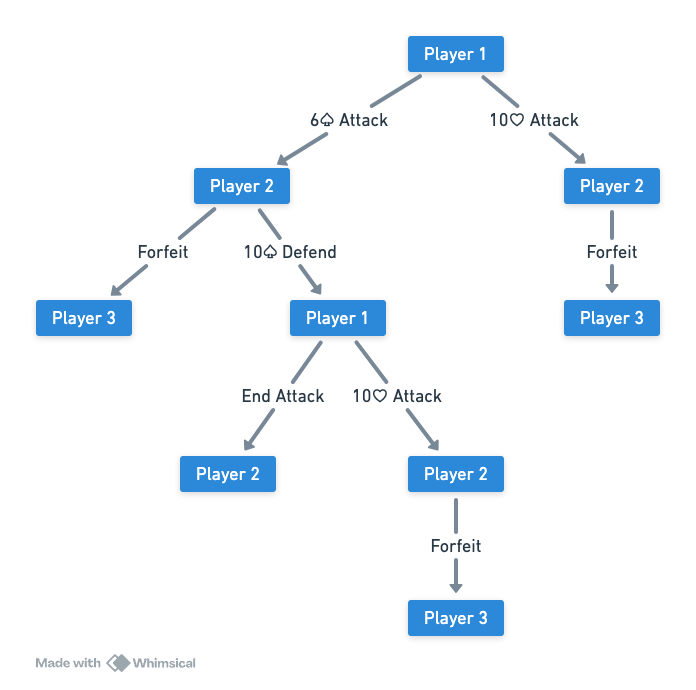
\includegraphics[width=8cm]{gametree.png}
	\caption{A basic cutting of a game tree of Durak, where Player 1 (the attacker) has 6 Spades, 10 Hearts and Player 2 has 10 Spades, 8 Hearts.}
	\label{fig:gametree}
\end{figure}

\(max^n\) is a decision-making algorithm for simulating possible future game states and evaluating them based on a scoring function. There is a vector of payoffs for each position, where each payoff corresponds personally to each player. Every player will aim to maximise their individual payoff to exit the game early and win.

The figure is a simple example of how Durak is represented in nodes. The scenario only has 2 cards, but typical games are played with up to 6.

Here's a breakdown of \(max^n\) in the context of Durak attacking:

\begin{lstlisting}
function maxnAttack(depth, maxDepth, gameState)
  if depth == maxDepth or gameIsOver(gameState)
    return (EndAttack, evaluateState(gameState))
  else
    newState = deal cards if needed and filter out winners
    possibleActions = generateAttackActions(gameState')
    
    results = []
    
    for each action in possibleActions
      newState = applyAttackAction(gameState', action)
      
      // Recursively call maxnDefend to simulate defender's response
      (opponentAction, scores) = maxnDefend(depth + 1, maxDepth, newState)
      results.append((action, scores))
    
    // Find the action with the best score for the attacker (maximum score for attacker's ID)
    bestResult = maximumBy(results, key=lambda result: result[1][playerId])

    return bestResult
\end{lstlisting}

The maxnDefend functionality would be similar to the above, but it finds the maximum of that defender's payoff.


The evaluation function used is a negative of how many cards each player is left with, giving double the value to the trump cards. The aim is to have no cards, so a negative of card count would give lighter hands a better value. It also uses the strategies found by Bonnet\cite{bonnet}. When a player's cards can all be beaten by another in the same rank, this is a weakness and their count is added. It is left to the reader to potentially find an even better evaluation function, one that could even include cooperation to avoid being the 1 loser.

\begin{figure}[h]
	\centering
	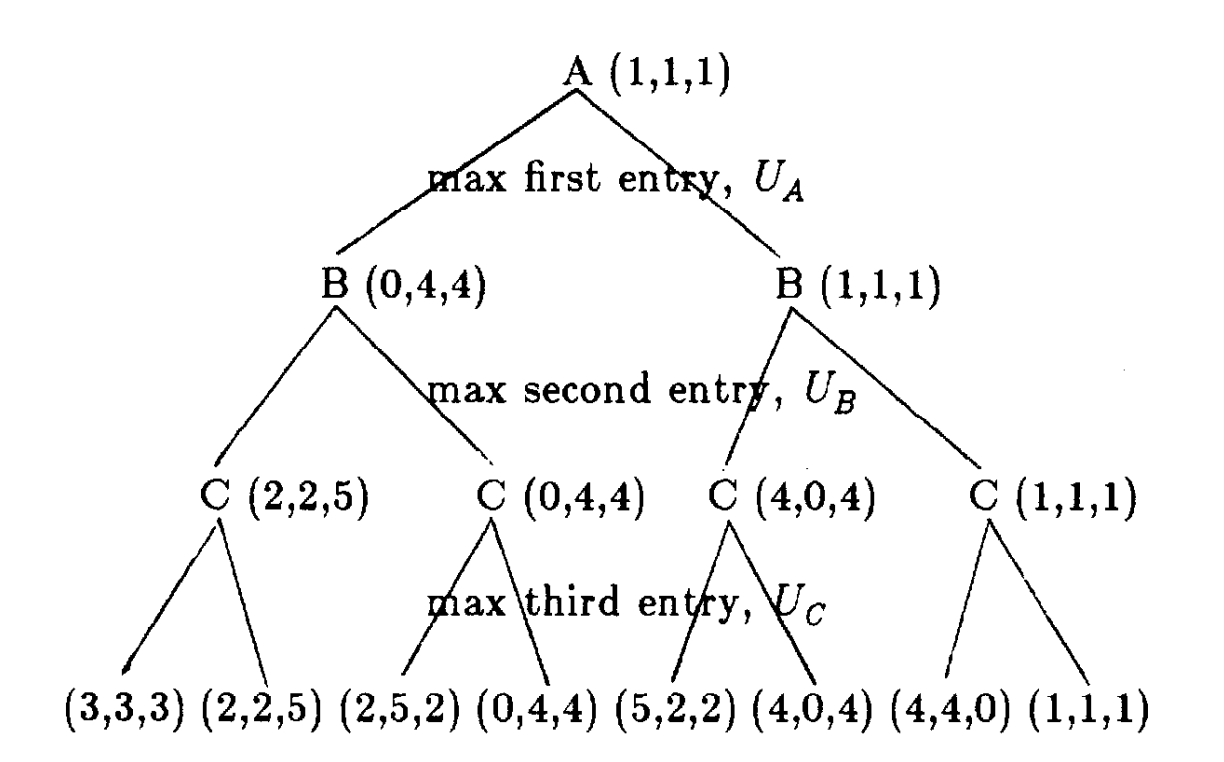
\includegraphics[width=8cm]{maxn.png}
	\caption{A representation of max n, provided by Luckhart\cite{luckhart}}
	\label{fig:maxn}
\end{figure}

\chapter{Conclusion and Future Work}

\(max^n\) is the optimal strategy for n-player card games out of the three. To evaluate in games of 4--6 players, the three strategies mentioned in this paper were randomly assigned as players. The \(max^n\) function had won 94\% of its games over 500, although this will massively vary depending on eval functions. Future work could include cooperation of players and Reinforcement Learning


\bibliographystyle{vancouver}
\bibliography{sources}

\end{document}